\documentclass[aspectratio=169]{beamer}
\usepackage{graphicx}

% Add slide numbers
% Custom footline with slide numbers in bottom left
\setbeamertemplate{footline}{
  \hspace{1em}% Add some left margin
  \usebeamercolor[fg]{page number in head/foot}%
  \usebeamerfont{page number in head/foot}%
  \insertframenumber\,/\,\inserttotalframenumber%  Format: "current / total"
  \vskip2pt%  Small vertical spacing
}

\beamertemplatenavigationsymbolsempty

\begin{document}

\begin{frame}
  \frametitle{Quantization Noise in ADCs}
  \begin{center}
    \includegraphics[height=0.7\textheight,keepaspectratio]{../../build/qnoise.pdf}
    \vspace{1em}

    $\displaystyle \sigma_{V_{\mathrm{qnoise}}} = \frac{2 V_\mathrm{ref}}{2^N \sqrt{12}}$
  \end{center}
\end{frame}

\begin{frame}
  \frametitle{Two-Column Example}

  \begin{columns}
    % Left column with equations and small image
    \begin{column}{0.5\textwidth}
      % Capacitance densities for 1, 2, and 3 layers (in fF/$\mu$m$^2$)
      1 layer: $?~\mathrm{fF}/\mu\mathrm{m}^2$ \\
      2 layers: $?~\mathrm{fF}/\mu\mathrm{m}^2$ \\
      3 layers: $?~\mathrm{fF}/\mu\mathrm{m}^2$ \\
      % Pelgrom matching coefficient for 65nm CMOS
      Matching coefficient: $\sigma(\Delta C/C) = 0.85\% \times \sqrt{C~[\mathrm{fF}]}$
      \vspace{2em}
      % Small square image at the bottom, centered
      \begin{center}
        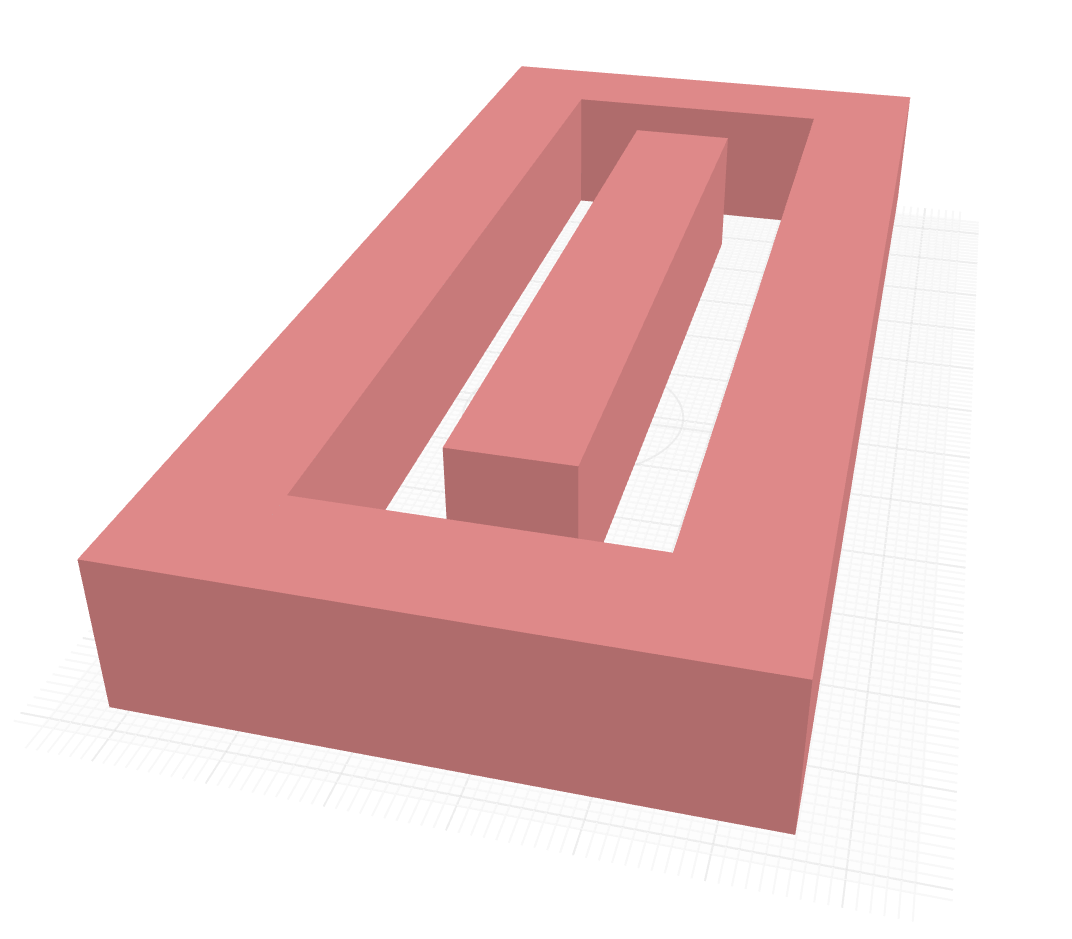
\includegraphics[width=\linewidth,height=0.4\textheight,keepaspectratio]{../images/cdac_unit_cell_3d.png}
      \end{center}
    \end{column}

    % Right column with large image, centered
    \begin{column}{0.5\textwidth}
      \begin{center}
        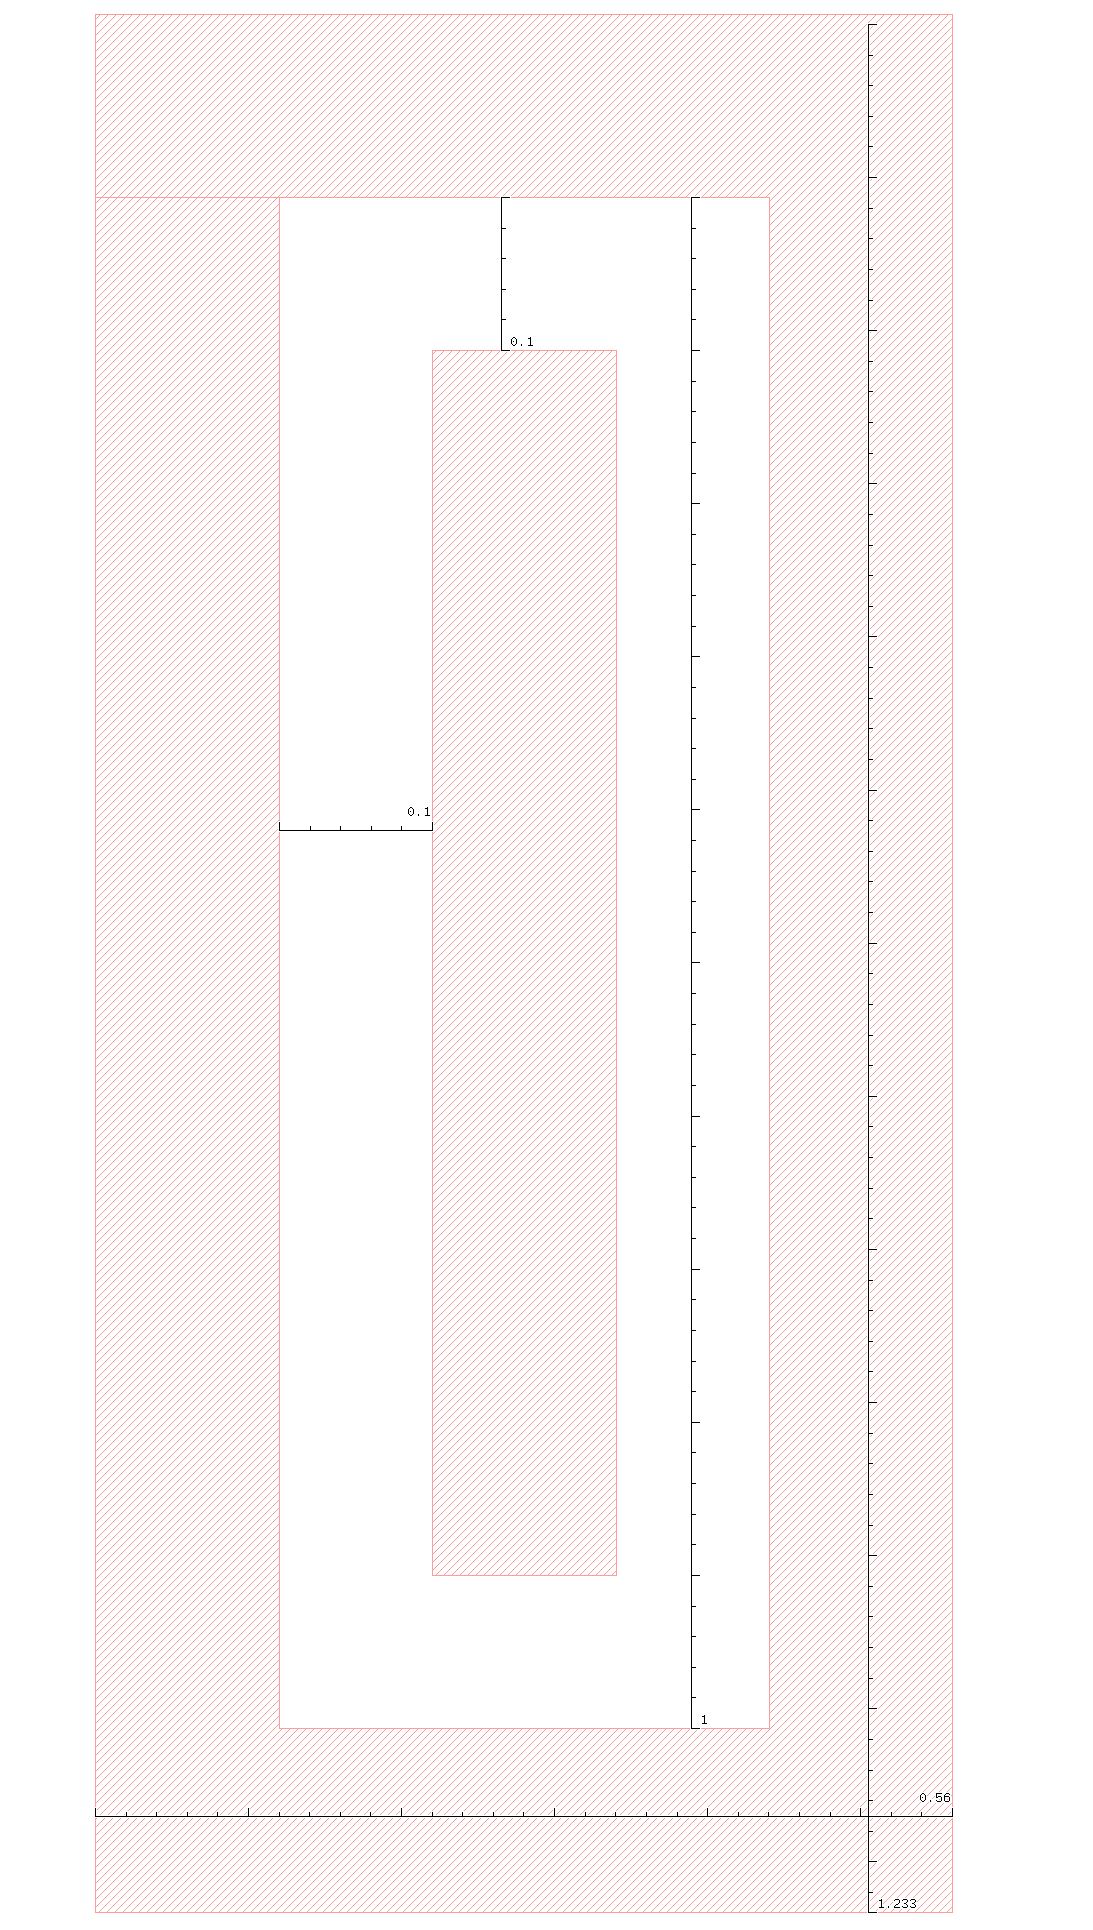
\includegraphics[width=\linewidth,height=0.8\textheight,keepaspectratio]{../images/cdac_unit_cell.png}
      \end{center}
    \end{column}

  \end{columns}

\end{frame}


\begin{frame}
  \frametitle{CDAC Array Overview}

  \begin{columns}
    % Left column: math and small image
    \begin{column}{0.5\textwidth}
      % Math section at the top
      \[
        \text{Total Area} = 1940~\mu\mathrm{m}^2
      \]
      % Small square image at the bottom, centered
      \begin{center}
        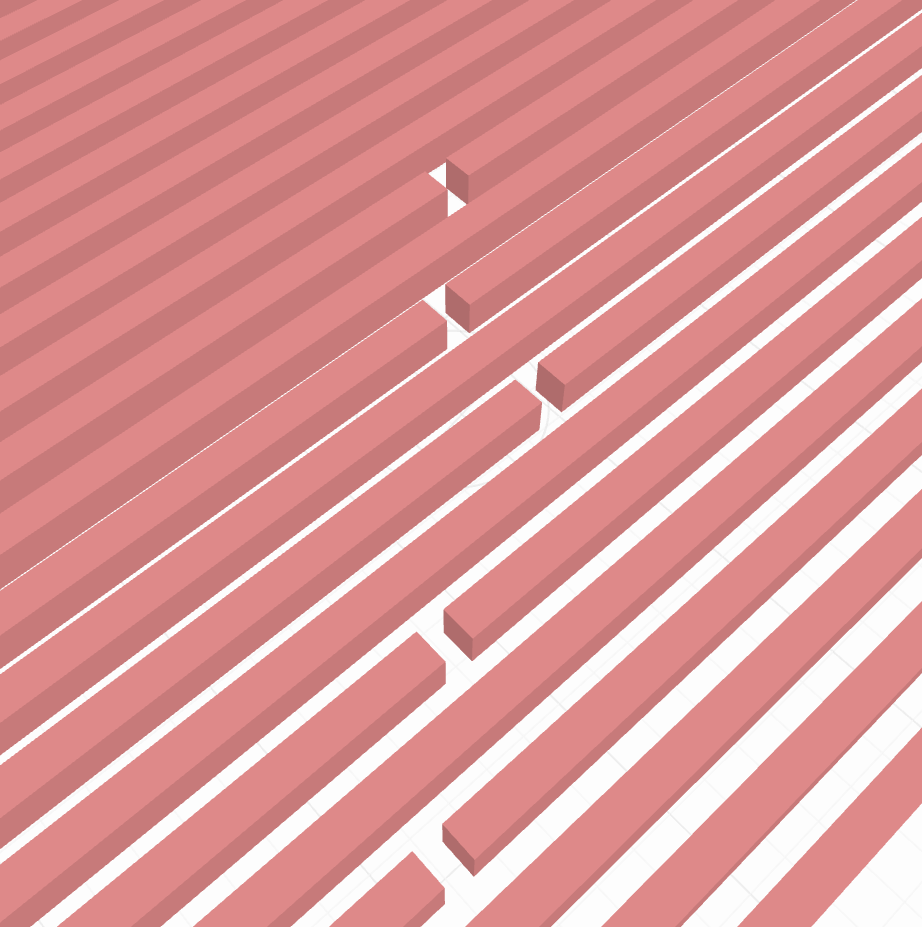
\includegraphics[width=\linewidth,height=0.5\textheight,keepaspectratio]{../images/cdac_array_3d.png}
      \end{center}
    \end{column}

    % Right column: large image, centered
    \begin{column}{0.5\textwidth}
      \begin{center}
        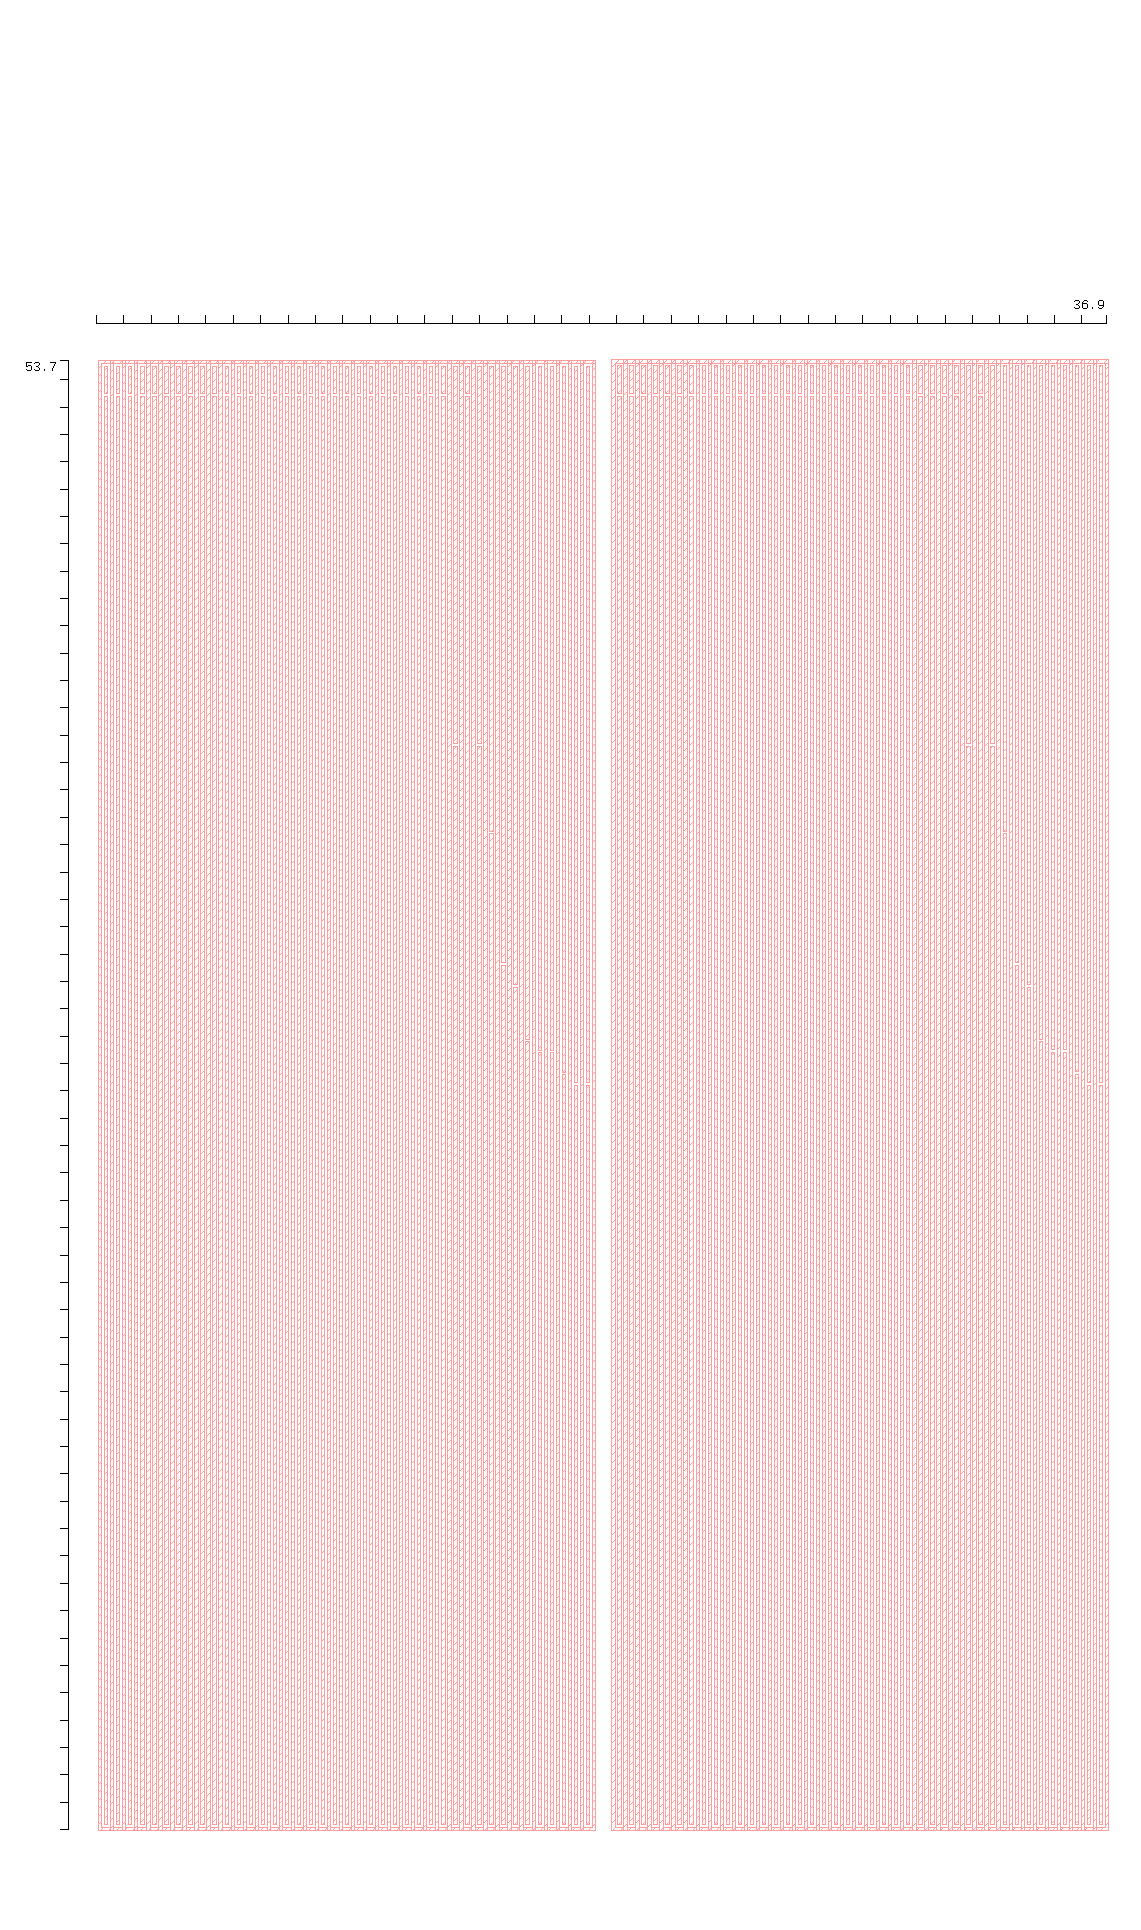
\includegraphics[width=\linewidth,height=0.85\textheight,keepaspectratio]{../images/cdac_array.png}
      \end{center}
    \end{column}
  \end{columns}

\end{frame}

\end{document}